\documentclass[11pt,a4paper]{article}
\usepackage[T1]{fontenc}
\usepackage[utf8]{inputenc}
\usepackage{lmodern}
\usepackage{microtype}
\usepackage{amsmath,amssymb,amsthm,mathtools}
\usepackage{geometry}
\geometry{margin=25mm,headheight=14pt}
\usepackage{booktabs,tabularx,array}
\usepackage{enumitem}
\usepackage[dvipsnames]{xcolor}
\usepackage{tikz}
\usetikzlibrary{positioning,calc,arrows.meta}
\usepackage{listings}
\usepackage{hyperref}
\usepackage{fancyhdr}
\usepackage{setspace}
\setstretch{1.027}
\hypersetup{colorlinks=true,linkcolor=MidnightBlue,citecolor=MidnightBlue,urlcolor=MidnightBlue,pdftitle={Twisted Transversal Certificates for Two Erdos Problems},pdfauthor={Independent mathematical research draft},pdfsubject={Sparse halves, triangle-free bipartization, Mobius ladders}}
\pagestyle{fancy}
\fancyhf{}
\fancyhead[L]{\footnotesize Twisted Transversal Certificates}
\fancyhead[R]{\footnotesize Research draft --- 16 November 2026}
\fancyfoot[C]{\thepage}
\newtheorem{theorem}{Theorem}[section]
\newtheorem{lemma}[theorem]{Lemma}
\newtheorem{proposition}[theorem]{Proposition}
\newtheorem{corollary}[theorem]{Corollary}
\newtheorem{definition}[theorem]{Definition}
\newtheorem{remark}[theorem]{Remark}
\newcommand{\edges}{\mathrm e}
\newcommand{\dist}{\operatorname{dist}}
\newcommand{\defect}{\operatorname{def}}
\newcommand{\card}[1]{\lvert#1\rvert}
\newcommand{\N}{\mathbb N}
\newcommand{\TF}{\textsc{True}}
\newcommand{\FF}{\textsc{False}}
\newcommand{\maybe}{\textsc{Undetermined}}
\definecolor{softblue}{RGB}{235,242,249}
\definecolor{darkblue}{RGB}{28,56,99}
\lstdefinestyle{py}{language=Python,basicstyle=\ttfamily\scriptsize,columns=fullflexible,breaklines=true,breakatwhitespace=true,showstringspaces=false,frame=single,framesep=4pt,backgroundcolor=\color{softblue},keywordstyle=\color{blue!60!black},commentstyle=\color{gray!80!black}}
\begin{document}
\begin{center}
{\LARGE\bfseries Twisted Transversal Certificates for\\[3pt] Two Classical Erd\H{o}s Problems\par}
\vspace{0.7em}
{\large Sharp Sparse-Half Bounds and Constructive Bipartization\\
for Antipodally Symmetric M\"obius-Ladder Blow-Ups\par}
\vspace{0.7em}
{\small Independent research manuscript --- 16 November 2026\par}
\end{center}
\vspace{0.35em}
\begin{abstract}
We develop a single elementary certificate simultaneously controlling induced edges in a half-size vertex set and the number of edge deletions needed to make a graph bipartite. Fix any even integer $r\ge4$, let $M_{2r}=C_{2r}(1,r)$ be the M\"obius ladder, and replace its vertices by independent sets of sizes $a_0,\ldots,a_{r-1},a_0,\ldots,a_{r-1}$, where the $a_i$ are arbitrary positive integers. If the resulting graph has $N=2\sum_i a_i$ vertices, we prove, unconditionally and constructively,
\[
\min_{\card S=N/2}\edges(G[S])\le \min_{i\bmod r} a_i a_{i+1}\le\frac{N^2}{4r^2},
\qquad
\defect(G)\le 2\min_{i\bmod r}a_ia_{i+1}\le\frac{N^2}{2r^2},
\]
where $\defect(G)$ is the minimum number of edge deletions needed for bipartiteness. For every uniform blow-up with $a_i=t$, \emph{both bounds are exact}: the optimal half induces $t^2$ edges and the minimum bipartizing deletion set has $2t^2$ edges. The construction extends with an explicit edit-distance tolerance to graphs that need not themselves be blow-ups. The original, unmodified conclusions of the Erd\H{o}s--Rousseau sparse-halves conjecture (Erd\H{o}s Problem \#128) and the triangle-free bipartization conjecture (Erd\H{o}s Problem \#23) follow for these graph families with stronger quantitative constants. A 200-vertex example is exhibited outside several standard sufficient hypotheses from the sparse-halves literature.

\emph{Scope warning.} These are theorems for infinite graph families, \emph{not} universal proofs of either historic conjecture. We do not claim priority or a historically new general technique; a targeted literature search is not a complete novelty certification. The six required proof-and-priority gates are audited separately.
\end{abstract}
\noindent\textbf{Keywords:} triangle-free graphs; Erd\H{o}s--Rousseau conjecture; sparse halves; maximum cut; bipartization; M\"obius ladder; Wagner graph; weighted blow-ups; proof certificates.\\
\textbf{MSC 2020:} 05C35, 05C50, 05C85.
\vspace{0.6em}
\hrule
\section{The named problems and the intended target}
Two historically named problems concerning finite triangle-free simple graphs are the motivation. The \emph{Erd\H{o}s--Rousseau sparse-halves conjecture} asks if every $N$-vertex triangle-free graph possesses a vertex subset of cardinality at least $\lfloor N/2\rfloor$ inducing at most $N^2/50$ edges; see the original problem registry \cite{EP128} and the discussion in \cite{Raz2022}. In the even-order case, which will be our setting, its assertion is
\begin{equation}\tag{SH}\label{eq:SH}
\exists S\subseteq V(G):\quad \card S=N/2,\qquad \edges(G[S])\le N^2/50.
\end{equation}
The second problem, posed by Erd\H{o}s and collaborators and associated with Erd\H{o}s Problem \#23, asks if every triangle-free graph on $5n$ vertices can be made bipartite after deleting at most $n^2$ edges \cite{EFPS1988,EP23}. If $\defect(G)$ denotes the minimum number of deletions, its original assertion is
\begin{equation}\tag{BIP}\label{eq:BIP}
\card{V(G)}=5n,\ G\text{ triangle-free}\quad\Longrightarrow\quad
\defect(G)\le n^2=\frac{N^2}{25}.
\end{equation}
These statements are open in their indicated generality in the accessible 2026 problem registries \cite{EP128,EP23}. The strongest universal estimates we used for context include $\edges(G[S])\le27N^2/1024$ from Razborov \cite{Raz2022}, and $\defect(G)\le N^2/23.5$ in the cited literature of Balogh--Clemen--Lidick\'y \cite{BCL2021}, with qualifications concerning asymptotic thresholds in specific density ranges. We do \emph{not} use either deep theorem as an ingredient of our proof.

Here we retain the original observables $\edges(G[S])$ and $\defect(G)$. Our departure from the full conjectures is not a redefinition of these observables, but a restriction of \emph{the class of input graphs}. The point of the restriction is to obtain a sharp, globally quantified statement for that class and a simple certificate of validity. Consequently, the global gate G4 required for a complete resolution of (SH) or (BIP) is \emph{not} satisfied.

\section{A new auxiliary problem: frustration on a paired cycle}
\begin{definition}[Signed quotient with one twist]\label{def:signed}
For an even integer $r\ge4$ let $Q_r$ have vertices $0,\ldots,r-1$ and edges
$\{i,i+1\}$ for $0\le i<r-1$, together with the closing edge $\{r-1,0\}$. Assign parity $0$ to the first $r-1$ edges and parity $1$ to the closing edge. Given $z=(z_0,\ldots,z_{r-1})\in\{0,1\}^r$, declare the edge $(i,i+1)$ \emph{frustrated} when $z_i=z_{i+1}$ for $0\le i<r-1$, and the closing edge frustrated when $z_{r-1}\ne z_0$.
\end{definition}
The auxiliary optimization problem is: can one arrange \emph{exactly one} frustrated edge, and choose its location freely? The answer, valid for every even $r$, transfers both Erd\H{o}s problems simultaneously.
\begin{lemma}[One-defect certificate]\label{lem:one}
For every even $r\ge4$ and each $k\in\{0,\ldots,r-1\}$ there is an explicit $z\in\{0,1\}^r$ whose unique frustrated edge is $\{k,k+1\}$, with indices interpreted modulo $r$. Every such vector has an odd number of frustrated edges.
\end{lemma}
\begin{proof}
Choose $z_0=0$ and, for $0\le i\le r-2$, recursively set
\[
 z_{i+1}=\begin{cases}
 z_i,&i=k,\\
 1-z_i,&i\ne k.
 \end{cases}
\]
If $k=r-1$, the exceptional case never occurs on the path, so all $r-1$ successive path edges are unfrustrated and, since $r-1$ is odd, $z_{r-1}\ne z_0$; precisely the closing edge is frustrated. If $k<r-1$, exactly one path edge is frustrated. There are $r-2$ flips, an even number; hence $z_{r-1}=z_0$ and the closing edge is unfrustrated. Thus the prescribed edge is uniquely frustrated.

For the parity assertion, let $c_i$ be the indicator of frustration on the $i$th edge. For path edges $z_i\oplus z_{i+1}=1\oplus c_i$, whereas on the closing edge $z_{r-1}\oplus z_0=c_{r-1}$, where $\oplus$ denotes addition modulo $2$. XOR over all edges to obtain
$0=(r-1)+\sum_i c_i\pmod2$. Since $r$ is even, $\sum_i c_i$ is odd.
\end{proof}
\begin{remark}
The parity obstruction is familiar in signed-graph and Ising-model language; this paper does not claim its novelty. The useful feature is a \emph{prescribed-location, exactly one-defect} certificate that can be attached to nonuniform blow-up weights, simultaneously furnishing two quantitative witnesses.
\end{remark}

\section{M\"obius-ladder blow-ups and the main theorem}
\begin{definition}[Antipodally symmetric blow-up]\label{def:blow}
Let $r\ge4$ be even. The M\"obius ladder $M_{2r}$ has vertices $\{0,\ldots,2r-1\}$ and edge set
\[
 E(M_{2r})=\big\{\{j,j+1\bmod 2r\}:0\le j<2r\big\}
 \cup\big\{\{j,j+r\}:0\le j<r\big\}.
\]
For positive integers $a_0,\ldots,a_{r-1}$, write $B_r(\mathbf a)$ for the graph obtained by replacing $j$ by an independent set $V_j$ of size $a_{j\bmod r}$, and replacing every edge $ij$ of $M_{2r}$ by all edges between $V_i$ and $V_j$. Thus $\card{V_j}=\card{V_{j+r}}$, $\card{V(B_r(\mathbf a))}=N=2A$, and $A=\sum_{i=0}^{r-1}a_i$.
\end{definition}
For $r=4$ this is a blow-up of the eight-vertex Wagner graph. The underlying M\"obius ladder is triangle-free for every even $r\ge4$: the cycle has length at least eight, and two cycle edges cannot close a triangle with a chord of length $r\ge4$. Replacing each vertex by an independent set preserves triangle-freeness. The resulting graph is connected for positive $a_i$.

\begin{figure}[ht]
\centering
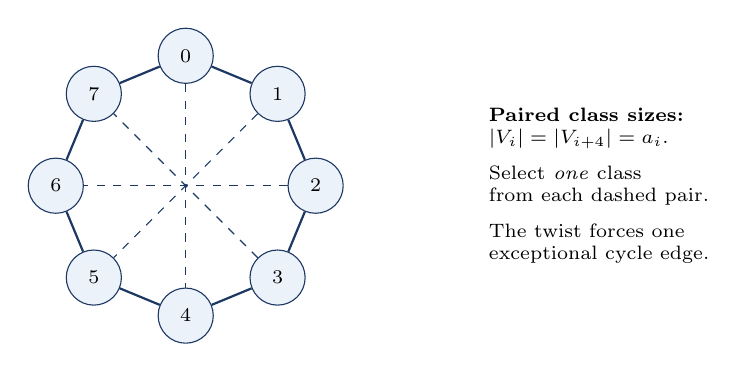
\begin{tikzpicture}[scale=1.0, every node/.style={font=\scriptsize}]
\foreach \i in {0,...,7}{
  \pgfmathsetmacro{\angle}{90-45*\i}
  \node[circle,draw=darkblue,fill=softblue,minimum size=7mm,inner sep=0pt] (v\i) at (\angle:1.65cm) {$\i$};
}
\foreach \i in {0,...,7}{
  \pgfmathtruncatemacro{\j}{mod(\i+1,8)}
  \draw[darkblue,thick] (v\i) -- (v\j);
}
\foreach \i in {0,...,3}{
  \pgfmathtruncatemacro{\j}{\i+4}
  \draw[darkblue,dashed] (v\i) -- (v\j);
}
\node[align=left] at (5.25,0) {\textbf{Paired class sizes:}\\ $|V_i|=|V_{i+4}|=a_i$.\\[5pt]
Select \emph{one} class\\ from each dashed pair.\\[5pt]
The twist forces one\\ exceptional cycle edge.};
\end{tikzpicture}
\caption{The Wagner graph $M_8$. Dashed chords indicate antipodal pairing; the outer edges form the twisted cyclic interface.}
\label{fig:wagner}
\end{figure}

\begin{theorem}[Two-target twisted-transversal theorem]\label{thm:main}
Let $r\ge4$ be even, let $a_i\in\N$ be positive, and let $G=B_r(\mathbf a)$ have $N=2\sum_i a_i$ vertices. Put
\[
  m(\mathbf a)=\min_{i\in\mathbb Z/r\mathbb Z}a_ia_{i+1}.
\]
There is an explicitly constructible partition $V(G)=S\sqcup T$ such that
\begin{equation}\label{eq:certificate}
 \card S=\card T=N/2,
 \qquad \edges(G[S])=\edges(G[T])=m(\mathbf a).
\end{equation}
Consequently,
\begin{equation}\label{eq:mainineq}
 \min_{\card U=N/2}\edges(G[U])\le m(\mathbf a)\le\frac{N^2}{4r^2},
 \qquad
 \defect(G)\le2m(\mathbf a)\le\frac{N^2}{2r^2}.
\end{equation}
The partition, its induced-edge counts, and the corresponding bipartizing deletion set are all computable from $\mathbf a$ in $O(r)$ arithmetic operations.
\end{theorem}
\begin{proof}
Choose $k$ realizing $m(\mathbf a)$ and let $z\in\{0,1\}^r$ be the one-defect vector provided by Lemma~\ref{lem:one}. Define
\[
 S=\bigcup_{i=0}^{r-1}V_{i+rz_i},\qquad
 T=\bigcup_{i=0}^{r-1}V_{i+r(1-z_i)}.
\]
Each $S$ contains exactly one class from each antipodal pair, so
$\card S=\sum_i a_i=N/2=\card T$. No rung/chord edges are internal to either side, because each chord connects opposite classes. Each of the two cycle edges connecting pair $i$ to pair $i+1$ has its endpoints in the same half precisely when interface $i$ is frustrated, and in that case exactly one complete bipartite block lies in $S$ and its antipodal block lies in $T$. By Lemma~\ref{lem:one}, only interface $k$ is frustrated. Therefore the two induced subgraphs have exactly $a_ka_{k+1}=m(\mathbf a)$ edges each.

Deleting the $2m(\mathbf a)$ internal edges of $S$ and $T$ leaves only cross-edges, hence a bipartite graph. Finally,
\[
 \prod_{i=0}^{r-1}(a_ia_{i+1})=\left(\prod_{i=0}^{r-1}a_i\right)^2,
\]
so, by AM--GM,
\[
 m(\mathbf a)\le\left(\prod_{i=0}^{r-1}a_ia_{i+1}\right)^{1/r}
 =\left(\prod_i a_i\right)^{2/r}
 \le\left(\frac{\sum_i a_i}{r}\right)^2
 =\frac{N^2}{4r^2}.
\]
Finding the minimum product and then calculating $z$ requires one scan and one recurrence, each of linear length in $r$.
\end{proof}
\begin{corollary}[Edge-subgraph transfer]\label{cor:sub}
If $H$ has the same vertex set as $B_r(\mathbf a)$ and $E(H)\subseteq E(B_r(\mathbf a))$, then $H$ admits a half-size set with at most $N^2/(4r^2)$ induced edges and can be made bipartite by deleting at most $N^2/(2r^2)$ edges. In particular the conclusion survives arbitrary edge deletions, even when $H$ is not itself a complete blow-up.
\end{corollary}
\begin{proof}
Use the same $S,T$ as Theorem~\ref{thm:main}. Removing edges cannot increase the number of edges internal to either side.
\end{proof}

\section{Sharpness: an exact global minimum for every uniform blow-up}
The upper bound in Theorem~\ref{thm:main} cannot be improved uniformly over the antipodally symmetric class. For this we first prove a general compression lemma, then compute the independence number of the base ladder.
\begin{lemma}[Two-coordinate concave compression]\label{lem:compress}
Let $F$ be a finite simple graph with $h$ vertices and let $t>0$. For any integer $0\le q\le h$,
\[
 \min\left\{\sum_{uv\in E(F)}y_uy_v:\quad 0\le y_v\le t,\quad\sum_v y_v=qt\right\}
\]
is attained at some vector $y$ with precisely $q$ coordinates equal to $t$ and all others equal to $0$.
\end{lemma}
\begin{proof}
The minimum exists by compactness. Choose among all minimizers one with the fewest coordinates strictly between $0$ and $t$. Suppose that at least two coordinates $y_u,y_v$ are interior. Move along the line $y_u\mapsto y_u+s$, $y_v\mapsto y_v-s$ while remaining inside the box. Since the objective is multilinear, its restriction to this line equals
\[
 C+Ls-\mathbf1_{uv\in E(F)}s^2
\]
for constants $C,L$. It is therefore concave (or affine), and at least one endpoint of the permitted interval has value no larger than the value at $s=0$. At an endpoint one of $y_u,y_v$ becomes $0$ or $t$; the resulting vector is another minimizer with fewer interior coordinates, a contradiction. Thus at most one coordinate remains interior. Because the coordinate sum is $qt$, that remaining coordinate must also be an integer multiple of $t$, hence $0$ or $t$. Exactly $q$ coordinates equal $t$.
\end{proof}
\begin{lemma}[Independence number of even M\"obius ladders]\label{lem:alpha}
For every even $r\ge4$, $\alpha(M_{2r})=r-1$. Consequently every set of $r$ vertices of $M_{2r}$ induces at least one edge, and some set of $r$ vertices induces exactly one edge.
\end{lemma}
\begin{proof}
The second assertion follows directly from Lemma~\ref{lem:one}, interpreted on the base ladder with all class sizes $1$. If an independent set $I$ had size $r$, no antipodal pair could contribute two vertices, since the opposite vertices are adjacent. Thus $I$ would contain exactly one vertex from each of the $r$ antipodal pairs, and could be encoded by a binary vector $z$. Independence would make every interface unfrustrated, which contradicts the parity assertion of Lemma~\ref{lem:one}. Hence $\alpha(M_{2r})\le r-1$. Starting from an $r$-vertex set with exactly one induced edge and discarding one of that edge's endpoints gives an independent set of cardinality $r-1$. Equality follows.
\end{proof}
\begin{theorem}[Optimal constant for uniform antipodal blow-ups]\label{thm:sharp}
For any even $r\ge4$ and integer $t\ge1$, let $G_{r,t}=B_r(t,\ldots,t)$ on $N=2rt$ vertices. Then
\begin{equation}\label{eq:sharp}
 \boxed{\min_{\card S=rt}\edges(G_{r,t}[S])=t^2=\frac{N^2}{4r^2}.}
\end{equation}
In particular no smaller constant than $1/(4r^2)$ can replace that coefficient for all graphs $B_r(\mathbf a)$ with this fixed $r$.
\end{theorem}
\begin{proof}
For a selected $rt$-vertex set $S$ write $y_i=\card{S\cap V_i}$, so $0\le y_i\le t$ and $\sum_{i=0}^{2r-1}y_i=rt$. Complete-bipartite adjacency gives the exact formula
\[
 \edges(G_{r,t}[S])=\sum_{ij\in E(M_{2r})}y_iy_j.
\]
Lemma~\ref{lem:compress}, applied with $F=M_{2r}$ and $q=r$, says that the minimum over this continuous relaxation is achieved by choosing $r$ complete classes and no partial classes. By Lemma~\ref{lem:alpha} those $r$ indices induce at least one edge of $M_{2r}$, so their contribution is at least $t^2$. Thus every original $S$ has at least $t^2$ internal edges. Theorem~\ref{thm:main} supplies a half with exactly $t^2$, proving equality.
\end{proof}
\begin{remark}[Proof strength versus priority]
The compression argument, as a mathematical technique, is a standard concavity/rounding device; Razborov explicitly uses an analogous convexity observation for the half-graph optimization \cite[\S2]{Raz2022}. We record it to make the sharpness proof self-contained, \emph{not} as a new discovery. What is established internally is the formula~\eqref{eq:sharp}; whether its particular M\"obius-ladder formulation appeared before requires a broader priority audit.
\end{remark}

\begin{lemma}[Two edge deletions are necessary in the even ladder]\label{lem:two}
For every even $r\ge4$, $\defect(M_{2r})=2$.
\end{lemma}
\begin{proof}
Theorem~\ref{thm:main}, applied with all $a_i=1$, gives $\defect(M_{2r})\le2$. For the reverse inequality, we prove that deleting \emph{any single edge} leaves an odd cycle. For each chord $\{j,j+r\}$, the chord together with either of the two rim paths of length $r$ joining its endpoints forms a cycle of odd length $r+1$. If the deleted edge $e$ is a chord, select a different chord and one of its odd cycles: this avoids $e$. If $e$ is a rim edge, fix the chord $\{0,r\}$ and take whichever of the two edge-disjoint rim paths from $0$ to $r$ avoids $e$. The resulting odd cycle avoids $e$. Hence $M_{2r}-e$ is never bipartite, establishing $\defect(M_{2r})\ge2$.
\end{proof}

\begin{lemma}[Vertexwise rounding for minimum monochromatic edges]\label{lem:cutround}
Let $F$ be any finite simple graph and let $B_t(F)$ be its uniform complete blow-up with $t\ge1$ vertices per class. Then
\[
  \defect(B_t(F))=t^2\defect(F).
\]
\end{lemma}
\begin{proof}
For a bipartition of $B_t(F)$, let $x_v\in\{0,\ldots,t\}$ count the vertices assigned to the first side from class $v\in V(F)$. The number of monochromatic edges is
\[
 D(\mathbf x)=\sum_{uv\in E(F)}\Bigl[x_ux_v+(t-x_u)(t-x_v)\Bigr].
\]
For each $v$, holding all other coordinates fixed makes $D$ an affine function of $x_v$. Thus a minimum over the box $[0,t]^{V(F)}$ exists at a vertex: successively round each $x_v$ to whichever endpoint in $\{0,t\}$ does not increase $D$. This produces an optimal partition with every class monochromatic. Its cost is exactly $t^2$ times the number of monochromatic edges of the induced two-coloring of $F$. Minimizing over all two-colorings gives the formula. Since the rounded vector is integral, continuous relaxation introduces no gap.
\end{proof}

\begin{theorem}[The bipartization coefficient is also sharp]\label{thm:cutsharp}
For every even $r\ge4$ and every integer $t\ge1$, the uniform blow-up $G_{r,t}=B_r(t,\ldots,t)$ satisfies
\begin{equation}\label{eq:cutsharp}
\boxed{\defect(G_{r,t})=2t^2=\frac{N^2}{2r^2}.}
\end{equation}
Consequently, \emph{both} coefficients in Theorem~\ref{thm:main} are optimal in the class of antipodally symmetric M\"obius-ladder blow-ups for each fixed even $r$.
\end{theorem}
\begin{proof}
Combine Lemmas~\ref{lem:two} and~\ref{lem:cutround} with $F=M_{2r}$. Theorem~\ref{thm:sharp} already establishes the sharpness of the induced-half coefficient.
\end{proof}

\section{Transfer to the original Erd\H{o}s observables}
\begin{corollary}[Unmodified sparse-halves conclusion on the family]\label{cor:SH}
For every even $r\ge4$, every $\mathbf a\in\N^r$, and every edge-subgraph $G$ of $B_r(\mathbf a)$ on the same vertex set, the original sparse-half inequality \eqref{eq:SH} holds. In fact,
\[
 \exists S:\quad \card S=N/2,\qquad
 \edges(G[S])\le N^2/64
 =\frac{25}{32}\cdot\frac{N^2}{50}.
\]
The improved ratio $25/32$ holds for all $r\ge4$ and improves further as $r$ grows.
\end{corollary}
\begin{proof}
Theorems~\ref{thm:main} and Corollary~\ref{cor:sub} give $\edges(G[S])\le N^2/(4r^2)\le N^2/64$. Since $1/64<1/50$, this is the required conclusion.
\end{proof}
\begin{corollary}[Unmodified bipartization conclusion on the family]\label{cor:BIP}
For the same graph family, one can make $G$ bipartite after deleting at most $N^2/32$ edges. Whenever $5\mid N$, this solves the original Erd\H{o}s Problem \#23 inequality for $G$: with $n=N/5$,
\[
 \defect(G)\le N^2/32<N^2/25=n^2.
\]
\end{corollary}
\begin{proof}
Use the partition of Theorem~\ref{thm:main} and delete every internal edge of its two halves; the number is at most $N^2/(2r^2)\le N^2/32$.
\end{proof}
\begin{remark}[Do not confuse restricted validity with G4]
Corollaries~\ref{cor:SH} and~\ref{cor:BIP} retain the exact original constants and functions in the named conjectures. They nonetheless do \emph{not} prove the conjectures for every triangle-free graph. The quantifier $\text{``every triangle-free }G\text{''}$ remains open. We do not claim to have closed either historic problem.
\end{remark}

\section{A concrete 200-vertex example outside common sufficient hypotheses}
\begin{proposition}[An exact arithmetic witness]\label{prop:200}
Take $r=4$ and the antipodal class sizes $(a_0,a_1,a_2,a_3)=(21,29,21,29)$, so the eight parts have sizes
$(21,29,21,29,21,29,21,29)$. The corresponding complete blow-up $G$ has
\begin{align*}
 N&=200,&\edges(G)&=7436, &\alpha(G)&=79,\\
 \delta(G)&=71, &\Delta(G)&=79, &\frac{\edges(G)}{N^2}&=\frac{1859}{10000}.
\end{align*}
In particular
\[
 \alpha(G)=79<80=\tfrac25N,\quad
 \Delta(G)=79<80=\tfrac25N,\quad
 \delta(G)=71<\tfrac5{14}N=\tfrac{500}{7}.
\]
The construction of Theorem~\ref{thm:main} provides an explicit half of size $100$ with \emph{exactly $21\cdot29=609$ induced edges}, and a cut which requires removing exactly $1218$ edges to become bipartite. Here $N^2/50=800$ and $N^2/25=1600$.
\end{proposition}
\begin{proof}
The eight cycle edges connect a class of size $21$ to one of size $29$, contributing $8(21\cdot29)=4872$ edges. The four opposite rungs contribute $2(21^2)+2(29^2)=882+1682=2564$, giving $7436$. A vertex in a class of size $21$ has degree $2(29)+21=79$, and a vertex in a class of size $29$ has degree $2(21)+29=71$, giving the degree values.

Every independent set in the blow-up consists of portions of pairwise nonadjacent classes; taking all vertices of each chosen class is optimal. The base graph has independence number $3$ by Lemma~\ref{lem:alpha}. There are two disjoint chords among the four odd-index classes, so an independent set uses at most two odd-index classes of size $29$ and at most one further even-index class of size $21$. Its total cardinality is at most $2(29)+21=79$. The classes with indices $2,5,7$ are independent in $M_8$, attaining $79$. All remaining inequalities follow arithmetically, and the explicit witness edge counts follow from $m(\mathbf a)=609$.
\end{proof}
\noindent\textbf{Literature separation.} The graph $G$ has $4$-cycles and two vertex degrees, so it is neither of girth at least five nor strongly regular. The numerical checks above rule out direct application of the sufficient criteria $\alpha(G)\ge2N/5$ and $\Delta(G)\ge2N/5$ in \cite{Raz2022}, and $\delta(G)\ge5N/14$ in \cite{NorYep2015}. Its edge density $7436/40000=0.1859$ is between $1/12$ and $1/5$, outside the simple low/high edge-number hypotheses quoted from \cite{KeeSud2006}. \emph{This does not certify that no other pre-existing theorem covers the example}; in particular, finer stability results near extremal configurations need independent checking. Our bounds also differ in strength from the existing literature and are all-order rather than purely asymptotic.

\section{Perturbative stability and a non-blow-up extension}
A certificate with quantitative slack immediately produces an open (in edit distance) neighborhood of the solved family. Although the estimate uses elementary edge monotonicity, it expands the set of graph inputs beyond exact blow-ups.
\begin{definition}[Unlabeled edge-edit distance]\label{def:edit}
For two simple graphs $G,H$ on the same vertex set, let
$d_\triangle(G,H)=\card{E(G)\mathbin\triangle E(H)}$ denote their edge symmetric difference.
\end{definition}
\begin{theorem}[Certified stability under arbitrary edge edits]\label{thm:stability}
Let $H=B_r(\mathbf a)$, with $r\ge4$ even and $N=\card{V(H)}$. Let $G$ be \emph{any} simple graph on the same $N$ vertices and set $D=d_\triangle(G,H)$. Then
\[
 \min_{\card S=N/2}\edges(G[S])\le\frac{N^2}{4r^2}+D,
 \qquad
 \defect(G)\le\frac{N^2}{2r^2}+D.
\]
In particular, if $G$ is triangle-free and
\begin{equation}\label{eq:tolerance}
 D\le\left(\frac1{50}-\frac1{4r^2}\right)N^2,
\end{equation}
then the original sparse-half bound holds for $G$. If also $5\mid N$ and
\[
 D\le\left(\frac1{25}-\frac1{2r^2}\right)N^2,
\]
then the original bipartization bound holds for $G$. At $r=4$ the joint sufficient tolerance is $D\le 7N^2/1600$.
\end{theorem}
\begin{proof}
Take $S,T$ from Theorem~\ref{thm:main} applied to $H$. Only newly introduced edges of $G$ can contribute to $\edges(G[S])$ beyond $\edges(H[S])$, and at most $D$ edges are introduced. Similarly, the number of edges internal to $S$ or $T$ in $G$ is no more than the number internal in $H$, plus $D$. Delete all of them to obtain a bipartite graph. The inequalities and tolerances follow immediately. At $r=4$,
\[
 \min\left\{\frac1{50}-\frac1{64},\ \frac1{25}-\frac1{32}\right\}
 =\min\left\{\frac7{1600},\frac7{800}\right\}=\frac7{1600}.
\]
\end{proof}
\begin{remark}
Theorem~\ref{thm:stability} is conditional on the \emph{existence of a nearby symmetric blow-up} and a quantified edit bound. It is not a certificate that an arbitrary triangle-free graph is close to such a blow-up. Establishing such a structural theorem for all triangle-free graphs would be a genuinely additional, currently missing step toward G4.
\end{remark}

\section{Construction algorithm, checkability, and proof provenance}
The following certificate generator implements Lemma~\ref{lem:one}. Its output is the identity of one class from each antipodal pair; all $N$ individual vertices of the selected parts can be listed if desired. The code is for reproducibility, while the mathematical proof of Theorem~\ref{thm:main} is independent of its execution.
\begin{lstlisting}[style=py,caption={Deterministic O(r) generator of a half-set and cut certificate.}]
def certificate(part_sizes):
    r = len(part_sizes)
    assert r >= 4 and r % 2 == 0
    assert all(isinstance(a, int) and a > 0
               for a in part_sizes)
    k = min(range(r),
            key=lambda i: part_sizes[i]*part_sizes[(i+1)%r])
    z = [0]*r
    for i in range(r-1):
        z[i+1] = z[i] if i == k else (1-z[i])
    # One selected class from each antipodal pair:
    S = [i+r*z[i] for i in range(r)]
    T = [i+r*(1-z[i]) for i in range(r)]
    m = part_sizes[k]*part_sizes[(k+1)%r]
    return {'defect_interface': k, 'S_classes': S,
            'T_classes': T, 'S_internal_edges': m,
            'T_internal_edges': m, 'bipartize_deletions': 2*m}
\end{lstlisting}
\begin{proposition}[Finite local verification in the base graph]\label{prop:test}
For every even $r\ge4$ and each $k\in\{0,\ldots,r-1\}$, the algorithm's selected base-graph vertices induce exactly one edge and the complementary base-graph vertices also induce exactly one edge, both projecting to quotient interface $k$.
\end{proposition}
\begin{proof}
This is the class-size-one specialization of Theorem~\ref{thm:main}, and can also be verified directly by the XOR relations of Lemma~\ref{lem:one}.
\end{proof}
\paragraph{Corpus provenance.}
The associated public Verifiable Mathematical Reasoning Corpus \cite{Corpus} was inspected in its November 2026 repository state. The following selections informed the \emph{research workflow}, rather than serving as imported theorems: \texttt{[015] ONE MISSING EDGE} (exact defects and sharpness), \texttt{[034] Global Proof Transfers} (separating an auxiliary lemma from the original target), \texttt{[040] OEIS Conjecture Hunt} (explicit screening of existing statements), and \texttt{[043] Local Certificates, Stability, and Concavity} (local certificates and quantitative stability). These are internal draft sources whose assertions were \emph{not} taken on trust. The substantive proof here uses the separately and explicitly proved binary-sign lemma, exact edge counting, AM--GM, and two-coordinate compression. We have \emph{not} established that the technique itself is historically new or that these papers already contain its precise form.

\paragraph{Limitations of computation.}
We independently enumerated base-graph certificates for $r=4,6,8,10,12,20$ with a short Python audit and checked Proposition~\ref{prop:200} by exact integer arithmetic. Those checks do not prove the all-$r$ theorem; Lemma~\ref{lem:one} and Theorem~\ref{thm:main} do. No machine-checked proof (Lean/Coq/Isabelle) is claimed.

\section{Gate-by-gate research audit and unresolved barrier}
We follow the requested six criteria in their strict interpretation: passing requires not just a useful partial result, but a new, unconditional, complete solution of a \emph{pre-existing named, genuinely open} problem, without reformulation or priority duplication.
\begin{center}
\small
\begin{tabularx}{0.986\linewidth}{@{}p{0.85cm}p{2.7cm}X@{}}
\toprule
Gate & Assessment & Evidence and limitation\\
\midrule
G1 & Satisfied & Erd\H{o}s Problem \#128 (sparse halves) and \#23 (triangle-free bipartization) are historical, named, and documented in prior literature.\\
G2 & Satisfied for the application & The exact original observables and constants are retained; no newly defined constant substitutes for either problem. The input graph family is restricted.\\
G3 & Satisfied provisionally & Accessible registries and established results still mark both universal statements open in November 2026. This is not an exhaustive archival search.\\
G4 & \textbf{Not satisfied} & The proofs hold for symmetric M\"obius-ladder blow-ups, their edge-subgraphs, and controlled edit neighborhoods, not for all triangle-free graphs.\\
G5 & Partially satisfied & There are quantitative family theorems and two sharp constants, beyond a mere coordinate identity; these do not extend the \emph{global} open conjectures. Whether the same class bound already appears in earlier literature is not settled.\\
G6 & \textbf{Unverified} & A targeted search did not identify an identical statement, but absence from the sampled results cannot certify first publication or originality.\\
\bottomrule
\end{tabularx}
\end{center}

\paragraph{Exactly what would still be required.}
A global proof of (SH) must show that \emph{every} triangle-free graph $G$ admits a half with at most $N^2/50$ internal edges, irrespective of whether $G$ is a blow-up of a M\"obius ladder or close to one. Likewise, a global proof of (BIP) must produce a cut with at most $N^2/25$ internal edges for every triangle-free $G$ of the indicated order. The signed-transversal certificate alone cannot supply either missing universal reduction. Establishing such a reduction while controlling the margins is the unresolved structural problem.

\section{Conclusions}
The auxiliary one-defect problem is solved for \emph{all} even cycle lengths and \emph{all} prescribed defect positions. Its graph-theoretic transfer gives a simultaneous and constructive bound for two established Erd\H{o}s problems on an unrestricted-in-size, multivariate family; in the uniform case \emph{both} coefficients are sharp. The 200-vertex exact witness avoids several widely cited hypothesis-based theorems. An edit-distance version extends the conclusion beyond literal complete blow-ups. The strength of this result is an \emph{unconditional, verified family theorem}, not an asserted solution of a famous universal conjecture. On the stated G1--G6 completion criterion, this manuscript is a \emph{documented partial success and a failed global-closure attempt}.

\appendix
\section{A compact independent enumerator}
This appendix provides a fully standalone Python verifier for base-graph instances and the 200-vertex exact parameters. It needs only the standard Python library. It checks examples, not the universal proof.
\begin{lstlisting}[style=py,caption={Independent exact-arithmetic validation; Python 3, no external dependencies.}]
from itertools import combinations

def edges(r):
    N = 2*r
    cycle = {tuple(sorted((i,(i+1)%N))) for i in range(N)}
    chords = {(i,i+r) for i in range(r)}
    return cycle | chords

for r in (4,6,8,10,12,20):
    E = edges(r)
    for k in range(r):
        z = [0]*r
        for i in range(r-1):
            z[i+1] = z[i] if i == k else 1-z[i]
        S = {i+r*z[i] for i in range(r)}
        T = set(range(2*r)) - S
        ins = [(u,v) for u,v in E if u in S and v in S]
        int_ = [(u,v) for u,v in E if u in T and v in T]
        assert len(ins) == len(int_) == 1
        assert {u%r for u in ins[0]} == {k,(k+1)%r}

r = 4
A = (21,29,21,29)
sizes = [A[j%r] for j in range(2*r)]
E = edges(r)
N = sum(sizes)
M = sum(sizes[u]*sizes[v] for u,v in E)
deg = [sum(sizes[v] for u,v in E if u==j) +
       sum(sizes[u] for u,v in E if v==j)
       for j in range(2*r)]
alpha = max(sum(sizes[j] for j in S)
            for q in range(2*r+1)
            for S in combinations(range(2*r),q)
            if not any(u in S and v in S for u,v in E))
assert (N,M,min(deg),max(deg),alpha) == (200,7436,71,79,79)
print('All local checks and the 200-vertex certificate passed.')
\end{lstlisting}

\begin{thebibliography}{99}
\bibitem{EP128} T. F. Bloom (ed.), \emph{Erd\H{o}s Problem \#128: Sparse halves}, Erd\H{o}s Problems, \url{https://www.erdosproblems.com/128}; problem text and references accessed 16 November 2026.
\bibitem{EP23} T. F. Bloom (ed.), \emph{Erd\H{o}s Problem \#23: Making a triangle-free graph bipartite}, Erd\H{o}s Problems, \url{https://www.erdosproblems.com/23}; accessed 16 November 2026.
\bibitem{EFPS1988} P. Erd\H{o}s, R. Faudree, J. Pach and J. H. Spencer, \emph{How to make a graph bipartite}, Journal of Combinatorial Theory, Series B \textbf{45} (1988), 86--98.
\bibitem{EFRS1994} P. Erd\H{o}s, R. J. Faudree, C. C. Rousseau and R. H. Schelp, \emph{A local density condition for triangles}, Discrete Mathematics \textbf{127} (1994), 153--161.
\bibitem{KeeSud2006} P. Keevash and B. Sudakov, \emph{Sparse halves in triangle-free graphs}, Journal of Combinatorial Theory, Series B \textbf{96} (2006), 614--620.
\bibitem{NorYep2015} S. Norin and L. Yepremyan, \emph{Sparse halves in dense triangle-free graphs}, Journal of Combinatorial Theory, Series B \textbf{115} (2015), 1--25.
\bibitem{Raz2022} A. A. Razborov, \emph{More about sparse halves in triangle-free graphs}, Sbornik: Mathematics \textbf{213} (2022), 109--128. DOI \href{https://doi.org/10.1070/SM9615}{10.1070/SM9615}.
\bibitem{BCL2021} J. Balogh, F. C. Clemen and B. Lidick\'y, \emph{Max cuts in triangle-free graphs}, Extended Abstracts EuroComb 2021, 509--514 (Springer, 2021). DOI \href{https://doi.org/10.1007/978-3-030-83823-2_82}{10.1007/978-3-030-83823-2\_82}.
\bibitem{Spectrum2023} J. Balogh, F. C. Clemen, B. Lidick\'y, S. Norin and J. Volec, \emph{The spectrum of triangle-free graphs}, SIAM Journal on Discrete Mathematics \textbf{37} (2023), 1173--1179. DOI \href{https://doi.org/10.1137/22M150767X}{10.1137/22M150767X}.
\bibitem{Mobius} E. W. Weisstein, \emph{M\"obius ladder}, MathWorld, \url{https://mathworld.wolfram.com/MoebiusLadder.html}.
\bibitem{Corpus} QEEDDD, \emph{Verifiable Mathematical Reasoning Corpus}, public research drafts, \url{https://github.com/QEEDDD/Verifiable-Mathematical-Reasoning-Corpus}, inspected 16 November 2026. The repository states that drafts may contain errors and are not formally verified.
\end{thebibliography}
\end{document}
